\section{Design of BigSim}

\begin{figure}[t]
\centering
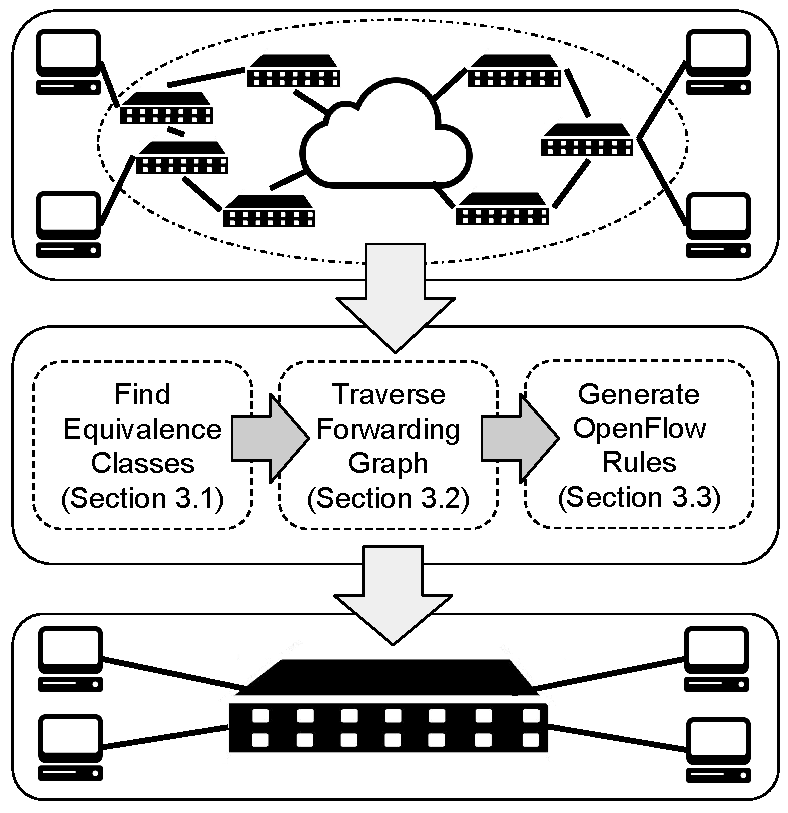
\includegraphics[scale=.6]{figures/BigSimOverview.pdf}
\caption{Overview of BigSim}
\label{Fig:BigSimOverview}
\end{figure}

We have sketched the process of how to replace a OpenFlow-switch-connected network
with a single OpenFlow switch in section~\ref{Sec:MotivationalExample}.

In this section, we elaborate the details and relevant algorithms
in each procedure.

\subsection{Finding Minimal Set of ECs}
By aggregating and slicing forwarding rules in a SDN network to ECs,
one can obtain a compact representation of all the classes of network flows.
\begin{definition}
Equivalence Class (EC) is the set of packets that
experience identical forwarding action at \textbf{any} network device.
\end{definition}
Inspired by VeriFlow\cite{Veriflow}, we aggregate forwarding rules using a trie
compositing by several sub-tries, each representing one header field.
In the tree-topology network, for example, the trie is just a single sub-trie that
corresponds to the packet header (network-layer destination address)
part of the rule match field.


\subsubsection{Disjoint EC as Disjoint Intervals}
By traversing from root node to a leaf node, we can obtain one set of packets
that a rule matches.
All the leaves thus contains all the rules in the network.
However, these rules are not independent and may overlapping with each other.
In essential, each rule is an range of packet header values;
the set of rules are thus a list of ranges $R$ where $\forall r \in R$ can be
described by a pair of starting header value and ending header value.
Finding the set of disjoint ECs requires us to splitting $R$ to
a list of non-overlapping intervals.
Not algorithmic described in\cite{Veriflow},
we show this task can be accomplished in $O(N \times M\log M)$ time,
where $M=|R|$ is the number of intervals and $N$ is the total number of header bits,
as follows\cite{SplitDisjointInterval}.

First we unzip $R$ into an array $A$ of $2M$ values,
each flagged as either a start $S$ or an end $E$ of a range.
\footnote{Equal values with same flag are reduced to an single element.}
Before iterating $A$, we sort it, breaking the tie by putting $S$ point before $E$ point.
Then we maintain the difference $d$ between the number of $S$ points and the number of $E$ points
seen so far, while visit each point in sorted order:
\begin{itemize}
\item If current element $x$ is $S$ and $d > 0$,
        we end the previous interval with ending value $x - 1$.
        start a new interval with starting value $x$
        (line~\ref{Alg:LineEndStart1}-\ref{Alg:LineEndStart2}).
\item If current element $x$ is $E$, we end the previous interval with ending value $x$.
        (line~\ref{Alg:LineEndEnd}).
\item In either case, we update the potential new interval's start value \textit{prev}
        (line~\ref{Alg:LineNewPrev1} and \ref{Alg:LineNewPrev2}).
\end{itemize}

Updating forwarding rules in the network will result in the change of EC set.
By maintaining the rules in a trie, we can efficiently update ECs incrementally as follows.
Inserting new rule to the trie require us to do a depth-first-style trie traverse.
This process automatically narrows down the affected rules by ignore the branches
that is impossible to overlap with the newly inserted rule.
The result of the procedure is the set of the effected ranges.
We only need to run Algorithm~\ref{Alg:GenDisjointECs} to update ECs in the effected ranges.

\begin{algorithm}[h]
\DontPrintSemicolon
\KwData{$R = $ set of rules from the leaf-node of the trie}
\KwResult{$EC = $ set of equivalence classes as disjoint intervals}
$cnt \gets 0$\;
$S = $ \{start points of $\forall r \in R\}$, $E = $ \{end points of $\forall r \in R\}$\;
$A \gets Sort(S \bigcup E)$ in non-decreasing order\;
$EC \gets \emptyset$\;
\ForEach {$x \in A$} {
        \uIf {$x \in S$} {
                \If {$cnt \neq 0$} {\label{Alg:LineEndStart1} 
                        $EC \gets EC \text{ }\bigcup \text{} [prev, x-1]$\;
                }\label{Alg:LineEndStart2} 
                $prev \gets x$\;\label{Alg:LineNewPrev1}
                $cnt \gets cnt + 1$\;
        }
        \Else ($x \in E$) {
                $EC \gets EC \text{ } \bigcup \text{ } [prev, x]$\;\label{Alg:LineEndEnd}
                $prev \gets x + 1$\;\label{Alg:LineNewPrev2}
                $cnt \gets cnt - 1$\;
        }
}
\caption{Generate Disjoint ECs\label{Alg:GenDisjointECs}}
\end{algorithm}

\subsubsection{Minimal EC Set}
The resulting disjoint EC set $ECS$ obtained from Algorithm~\ref{Alg:GenDisjointECs} are unfortunately not the optimal one with minimum size.
Many ECs can be merged together.
For example, EC1 and EC3 in section~\ref{Sec:MotivationalExample} can be seen as one EC.
By the definition of EC, since $\forall d$ takes identical forwarding action for any one of
the mergeable ECs, we have:
\begin{lemma}
A set of mergeable disjoint ECs has the same forwarding graph.
\label{Lemma:MergeFG}
\end{lemma}
Thus, operating on the minimal EC set can reduce running time in the later phase of
generating forwarding graph as well as populating final OpenFlow rules.
Here we provide a solution with its proof.
Our solution builds on the following Lemma.
\begin{lemma}
A pair of disjoint ECs in $ECS$ is mergeable if they intersect with
the same set of rules in the network.
\label{Lemma:MergeEC}
\end{lemma}
The proof of Lemma~\ref{Lemma:MergeEC} is as follows.
Let $\alpha$ and $\beta$ be two ECs that intersect with the same set of rules $\Delta$.
At $\forall$ network device $d$, let $\delta \in \Delta$ be the rule on $d$ with
highest priority.
If no such $\delta$ exist, packets from both $\alpha$ and $\beta$ are dropped on $d$.
Otherwise, device $d$ will forward packets from both $\alpha$ and $\beta$ according to the same
rule $\delta$.
By the definition of EC, packets in $\alpha$ and $\beta$ can be merged as one single EC
since at any network switch they have identical forwarding action.

Finding the list of rules $\Delta[\alpha]$ that intersects with EC $\alpha$ can be done
efficiently with two data structure,
each taking care one of the two cases\cite{FindIntersectionWiki}:
\begin{itemize}
\item Rule $\delta$ intersects $\alpha$ with its start and/or end point in $\alpha$.
        We can reuse the sorted array $A$ in Algorithm~\ref{Alg:GenDisjointECs}.
        Here we assume we augmented each value in $A$ with a pointer that points to
        the rule it belongs to.
        By doing binary search, we can find the minimum and maximum value in $A$ that
        are in the range of $\alpha$.
        All intervals that intersect with $\alpha$ must be contained between
        the minima and maxima.
        We can then do linear search in this reduced list of ranges $A'$,
        check one by one if the interval that value $a\in A'$ belongs to
        intersects with $\alpha$.
        The total time complexity for both linear and binary search is thus $O(\log M + K)$,
        assuming $K=|\Delta|$ is the number of reported intervals.
\item Rule $\delta$ covers $\alpha$ entirely. We can build
        a central interval tree\cite{ComputationalGeometryBook} using all available ranges.
        We pick a random value $x \in \alpha$ and query the central interval tree for
        all ranges that intersect with $x$, which can be done in $O(\log M + K)$ time,
        at the cost of $O(M log M)$ time for building the central interval tree. 
\end{itemize}

For each EC $\alpha$ we have found the list of intervals $\Delta[\alpha]$
that intersects with it with both interval tree and ordered list of boundary values.
By mapping each rule to an unique binary ID of length $\log_2 M$,
we can encode $\Delta[\alpha]$ to a string $C_\alpha$ of at most length $M\log_2 M$, putting
small binary IDs before large ones.
Then we use a hash table $H$ to group mergeable ECs by hashing each EC $x$ to $C_x$.
The minimal size of ECs is the number of unique keys in $H$.
In the later text, when we say ``iterate through all (disjoint) ECs" or "for each EC" etc,
we are actually visiting the first ECs in each set $H[key]$, $\forall key \in H$.


\subsection{Generating Forwarding Graphs}
In the second stage, we compute forwarding graphs for each EC and
compress them in order to be used in the next stage.
Forwarding graph not only concatenates the forwarding actions of each EC,
but also visualizes the flow the EC.
For a fixed EC $x$, we connect the network devices that have rules for $x$
with directed edges that point to the next hop,
which is available in the action field of the rule.
Since our goal is to compress the network logic, we are more interested in the sources
and sinks of the directed graph.

We define \textit{edge switches} as these switches whose port will be remapped to the port on
the resulting big switch;
in contrast, \textit{internal switches} are abstracted away in the final big switch.
Forwarding graphs are generated by starting from each \textbf{edge switch} and traversing
in the depth-first-search style by following the action of the highest-priority rule
covering EC $x$.
Source node $src$ and its out-going edge represent an edge switch $sw$ that
forwards EC $x$ \textbf{coming from} port $p$; it can be described by $(sw, p)$ pair.
Sink node $snk$ represent the end of the forwarding $sw$,
which is also denoted by $(sw, p)$, where $p$ is either the port number
specified by the action field or \texttt{NULL} if there is no rule for $x$ on $sw$.
%We denote the set of source nodes as $SRC(x)$, the set of sink nodes as $SNK(x)$.
Notice that (1) source nodes in $FG(x)$ can only be edge switch,
while it is possible that sink nodes are inner switches;
(2) the inner graph between sink and source may contain both edge and internal switches.

\begin{figure*}[t]
\centering
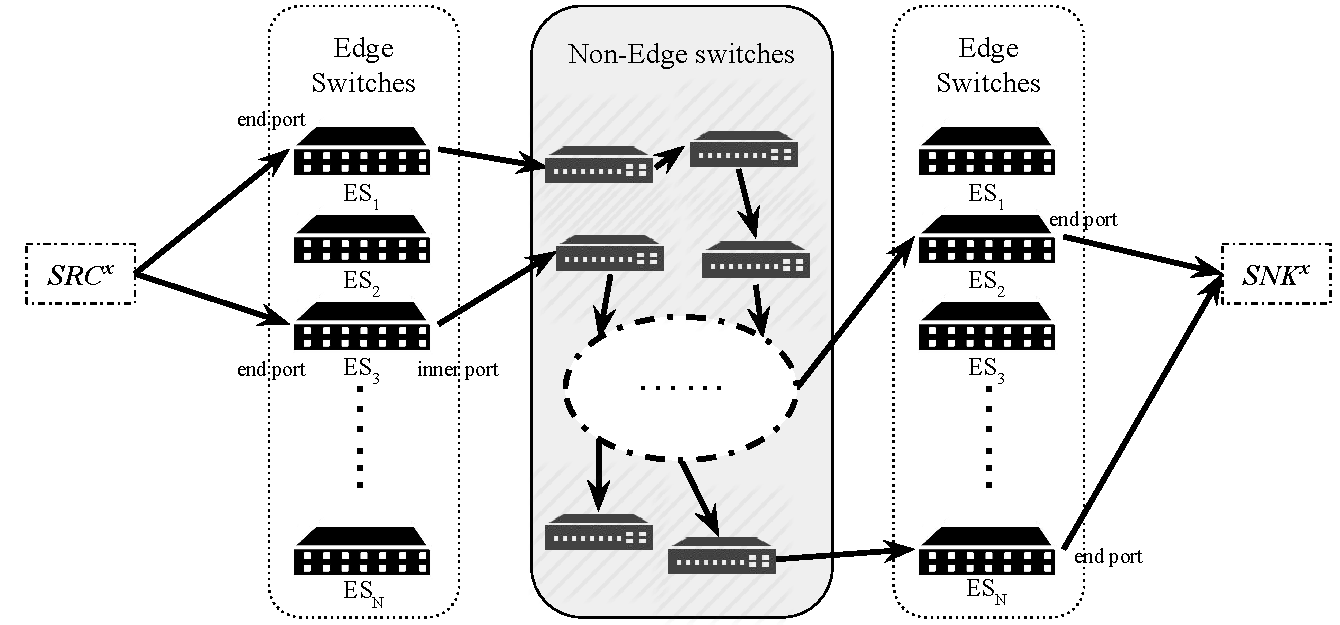
\includegraphics[scale=.75]{figures/ForwardingGraph.pdf}
\caption{An illustration of the $FG(x)$ forwarding graph for EC $x$}
\label{Fig:ForwardingGraphECX}
\end{figure*}

We depict the generalized forwarding graph $FG(x)$ for EC $x$
in Figure~\ref{Fig:ForwardingGraphECX}.
We add a super-source node $SRC^x$and a super-sink node $SNK^x$, both represent the EC $x$.
For convenience in discussion, we distinguish two kinds of port on \textbf{edge switch}es:
\textit{end port} connects to endpoints or the outside of the network we are abstracting, while
\textit{inner port} connects to another network device inside the network we are abstracting.
We add an edge from $SRC^x$ to a source node(edge switch) $src$ if
\begin{enumerate}
\item the edge switch has a forwarding rule $r$ that covers EC $x$;
\item the $IN\_PORT$ field of $r$ corresponds to an \textbf{end port} of the edge switch
\end{enumerate}
otherwise, we don't need to initiate traverse at all
(see line~\ref{Alg:LineStartDFS1} to \ref{Alg:LineStartDFS2}
in Algorithm~\ref{Alg:GenForwardingGraph}).
Correspondingly, we add an edge from a sink node $snk$ to super sink $SNK^x$
if both conditions are satisfied:
\begin{enumerate}
\item the sink node is representing an edge switch in the network;
\item the $OUT\_PORT$ field determined by the rule's action on the edge switch is \textbf{end port}
\end{enumerate}

Using the depth-first-search algorithm shown in Algorithm~\ref{Alg:GenForwardingGraph},
we can discover three kinds of ``path" in $FG(x)$ that related to rule generation on
the big virtual switch:
\begin{itemize}
\item \textbf{Forwarding Path}(line~\ref{Alg:LineForwardPath1}-\ref{Alg:LineForwardPath2}).
        The path, starting from super source,
        leads to super sink node through a end port on another edge switch to host.
        This is a normal forwarding path for packets $\in$ EC $x$.
\item \textbf{Dropped in the Middle}(line~\ref{Alg:LineDropPath1}-\ref{Alg:LineDropPath2}).
        The path ends inside the graph, unable to arrive
        at the super sink node. This path tell us that packets
        defined by EC $x$ are dropped, at least partially,
        in some intermediate switch in the network.
\item \textbf{Forwarding Loop}(line~\ref{Alg:LineLoopPath}).
        There is a directed cycle in the graph, which can be
        detected during the depth-first-search traverse.
        This behavior can be emulated in the semantic of \textbf{performance equivalence},
        but not by \textbf{logical equivalence} studied in this paper.        
        For example, we can emulate a forwarding loop in the network by
        (1) recording the volume of the looping packets;
        (2) increasing the delay of other packets on the basis of the amount of looping packets
        (3) adding a rule so that looping packets are dropped by big switch;
\end{itemize}

\begin{algorithm}[h]
\DontPrintSemicolon
\KwIn{$nodes = $ Switches that have rule for $x$ \newline
        Topology of the network $topo$}
\KwResult{Forwarding graph $FG(x)$ for EC $x$}
\SetKwProg{Fn}{Function}{}{\KwRet}
\SetKwFunction{Traverse}{traverse}
\SetKwFunction{GenRule}{generate\_rules}
\Fn{\Traverse{$curr$, $src$, $snk$}} {
        \uIf {$curr$ \upshape is \textbf{NOT} visited} {
                $r \gets$ \textbf{highest-priority} rule on $curr$ that covers $x$\;
                \If {r \upshape is NULL or $r.action$ is DROP} {\label{Alg:LineDropPath1}
                        $snk \gets$ ($curr$, NULL)\;
                        \GenRule{$x, src, snk$}\;
                        \KwRet\;
                }\label{Alg:LineDropPath2}
                $next \gets topo[curr][r.action.outport]$\;
                \If {next $\not\in$ nodes} {\label{Alg:LineForwardPath1}
                        $snk \gets$ ($curr$, $r.action.outport$)\;
                        \GenRule{$x, curr, src, snk$}\;
                        \KwRet\;
                }\label{Alg:LineForwardPath2}
                mark $curr$ as visited\;
                \Traverse{$next, src, snk$}\;
        }
        \Else {
                report forwarding loop\;\label{Alg:LineLoopPath}
        }
}\;
\ForEach{$n \in$ \upshape neighbors of $SRC^x$} {\label{Alg:LineStartDFS1}
        \If {\upshape $n$ is \textbf{NOT} visited} {
                $inport \gets$ inport number from $SRC^x$ to $n$\;
                \Traverse{$n$, $src=$\upshape($n$, $inport$), $snk=$NULL}\;
        }
}\label{Alg:LineStartDFS2}
\caption{Generate Forwarding Graph for EC $x$\label{Alg:GenForwardingGraph}}
\end{algorithm}


\subsection{Populating Flow Table on Big Switch}

Depending on the kind of path, we can easily generate OpenFlow rules on the abstracted
big switch at the end of forwarding graph traversal by calling \texttt{generate\_rules},
which is described in Algorithm~\ref{Alg:GenAllRules}.
We maintain a hash table $PortMap$ to map end ports on edge switches to the big virtual switch.
This table is configured as rule generation using $global\_port$ variable.
Algorithm~\ref{Alg:GenAllRules} fills the mandatory fields in an OpenFlow rule:
\begin{itemize}
\item The $MATCH$ field is given by the EC $x$ itself, e.g. the range of matching packets header
        (line \ref{Alg:LineMatch})
\item The $IN\_PORT$ field is the mapped port number of $src.port$ (line~\ref{Alg:LineInport})
\item Depending on the $dst$'s port, we generate either a drop action
        (line~\ref{Alg:LineGenDropRule})
        or a forward action with appropriate mapped port number of $dst.port$ 
        (line~\ref{Alg:LineGenForwardRule1}-\ref{Alg:LineGenForwardRule2})
\end{itemize}



\begin{algorithm}[h]
\DontPrintSemicolon
\KwData{$PortMap$ maps $port$ on $sw$ $\rightarrow port$ on big switch\newline
        $global\_port$ assigned to unseen port number}
\KwResult{New rule $r$ to install in $BS$}
Assume $global\_port$ is globally initialized to 0\;
\SetKwProg{Fn}{Function}{}{\KwRet}
\SetKwFunction{GenRule}{generate\_rules}
\Fn{\GenRule{$x, src, dst$}} {
        $r.match \gets x$\;\label{Alg:LineMatch}
        \If {src.port $\not\in$ PortMap[src.sw]} {
                $PortMap[src.sw][src.port] \gets global\_port++$\;
        }
        $r.inport = PortMap[src.sw][src.port]$\;\label{Alg:LineInport}
        \uIf {dst.port \upshape is NULL} {
                $r.action \gets $ drop\_action\;\label{Alg:LineGenDropRule}
        }
        \Else {
                \If {dst.port $\not\in$ PortMap[dst.sw]} {\label{Alg:LineGenForwardRule1}
                        $PortMap[dst.sw][dst.port] \gets global\_port++$\;
                }
                $r.action \gets $ forward\_action\;
                $r.action.outport \gets PortMap[dst.sw][dst.port]$\;\label{Alg:LineGenForwardRule2}
                
        }
}
\caption{Generate Rule for EC $x$ on Big Switch\label{Alg:GenAllRules}}
\end{algorithm}



